% article example for classicthesis.sty
\documentclass[10pt,a4paper]{article} % KOMA-Script article scrartcl
\usepackage{import}
\usepackage{xifthen}
\usepackage{pdfpages}
\usepackage{transparent}
\newcommand{\incfig}[1]{%
    \def\svgwidth{\columnwidth}
    \import{./figures/}{#1.pdf_tex}
}
\usepackage{lipsum}     %lorem ipsum text
\usepackage{titlesec}   %Section settings
\usepackage{titling}    %Title settings
\usepackage[margin=10em]{geometry}  %Adjusting margins
\usepackage{setspace}
\usepackage{listings}
\usepackage{amsmath}    %Display equations options
\usepackage{amssymb}    %More symbols
\usepackage{xcolor}     %Color settings
\usepackage{pagecolor}
\usepackage{mdframed}
\usepackage[utf8]{inputenc}
\usepackage{longtable}
\usepackage{multicol}
\usepackage{graphicx}
\graphicspath{ {./Images/} }
\setlength{\columnsep}{1cm}

% ====| color de la pagina y del fondo |==== %
\pagecolor{black}
\color{white}



\begin{document}
    %========================{TITLE}====================%
    \title{{  13th lab of Forensics  }}
    \author{{Rodrigo Castillo}}
    \date{\today}

    \maketitle


     % ====| Loguito |==== %
    
\includegraphics[width=0.1\linewidth]{negro_cara.png}
    %=======================NOTES GOES HERE===================%
    \section{captures}
    for the following task, i'll make one script that will execute all the
    commands listed on the table and then i'll explain every command on the
    table.
    The script...
    \begin{figure}[h!]
        \centering
        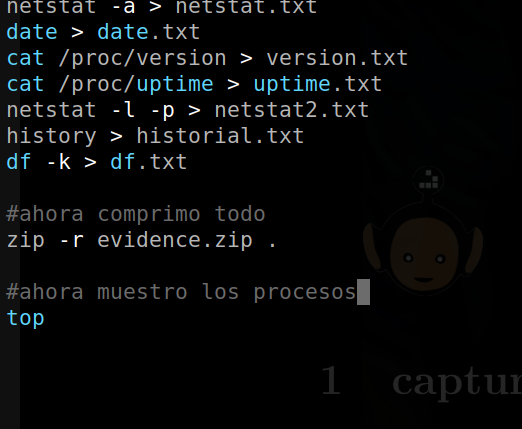
\includegraphics[width=0.5\linewidth]{script.png}
        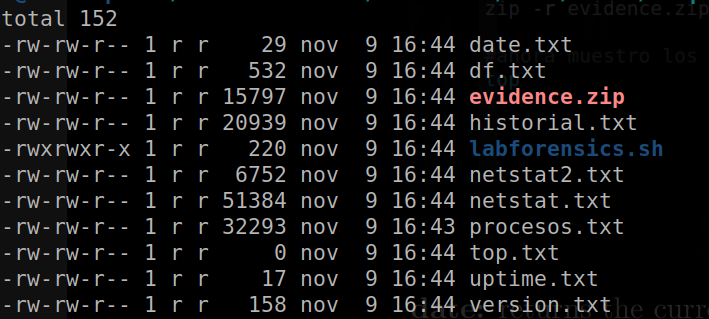
\includegraphics[width=0.5\linewidth]{result.png}
        \caption{script and result}
        \label{script}
    \end{figure}

    \textbf{date:} returns the current date .
    \\
    \textbf{df:} returns the current state of the disks .
    \\
    \textbf{history:} return the history of bash commands .
    \\
    \textbf{netstat:} return the current state of wireless conections.
    \\
    \textbf{top:} return the current processes running.
    \\
    \textbf{uptime}  return the cuantity of time that the machine has been on.
    \\
    \textbf{version} return the linux version.


















    %=======================NOTES ENDS HERE===================%

    % bib stuff
    \nocite{*}
    \addtocontents{toc}{{}}
    \addcontentsline{toc}{section}{\refname}
    \bibliographystyle{plain}
    \bibliography{../Bibliography}
\end{document}
